        %%******************************************%%
        %%                                          %%
        %%        Modello di tesi di laurea         %%
        %%            di Andrea Giraldin            %%
        %%                                          %%
        %%             2 novembre 2012              %%
        %%                                          %%
        %%******************************************%%


% I seguenti commenti speciali impostano:
% 1. 
% 2. PDFLaTeX come motore di composizione;
% 3. tesi.tex come documento principale;
% 4. il controllo ortografico italiano per l'editor.

% !TEX encoding = UTF-8
% !TEX TS-program = pdflatex
% !TEX root = tesi.tex
% !TEX spellcheck = en-EN

\documentclass[10pt,                    % corpo del font principale
               a4paper,                 % carta A4
               twoside,                 % impagina per fronte-retro
               openright,               % inizio capitoli a destra
               english,                                  
               ]{book}    

%**************************************************************
% Importazione package
%************************************************************** 

%\usepackage{amsmath,amssymb,amsthm}    % matematica


\usepackage[T1]{fontenc}                % codifica dei font:
                                        % NOTA BENE! richiede una distribuzione *completa* di LaTeX

\usepackage[utf8]{inputenc}             % codifica di input; anche [latin1] va bene
                                        % NOTA BENE! va accordata con le preferenze dell'editor

\usepackage[english]{babel}    % per scrivere in italiano e in inglese;
                                        % l'ultima lingua (l'italiano) risulta predefinita

\usepackage{bookmark}                   % segnalibri

\usepackage{caption}                    % didascalie

\usepackage{chngpage,calc}              % centra il frontespizio

\usepackage{csquotes}                   % gestisce automaticamente i caratteri (")

\usepackage{emptypage}                  % pagine vuote senza testatina e piede di pagina

\usepackage{epigraph}			% per epigrafi

\usepackage{eurosym}                    % simbolo dell'euro

%\usepackage{indentfirst}               % rientra il primo paragrafo di ogni sezione

\usepackage{graphicx}                   % immagini

\usepackage{hyperref}                   % collegamenti ipertestuali

\usepackage[binding=5mm]{layaureo}      % margini ottimizzati per l'A4; rilegatura di 5 mm

\usepackage{listings}                   % codici

\usepackage{microtype}                  % microtipografia

\usepackage{mparhack,fixltx2e,relsize}  % finezze tipografiche

\usepackage{nameref}                    % visualizza nome dei riferimenti                                      

\usepackage[font=small]{quoting}        % citazioni

\usepackage{subfig}                     % sottofigure, sottotabelle

%\usepackage[english]{varioref}          % riferimenti completi della pagina

\usepackage[dvipsnames]{xcolor}         % colori

\usepackage{booktabs}                   % tabelle                                       
\usepackage{tabularx}                   % tabelle di larghezza prefissata                                    
\usepackage{longtable}                  % tabelle su più pagine                                        
\usepackage{ltxtable}                   % tabelle su più pagine e adattabili in larghezza

\usepackage[toc, acronym]{glossaries}   % glossario
                                        % per includerlo nel documento bisogna:
                                        % 1. compilare una prima volta tesi.tex;
                                        % 2. eseguire: makeindex -s tesi.ist -t tesi.glg -o tesi.gls tesi.glo
                                        % 3. eseguire: makeindex -s tesi.ist -t tesi.alg -o tesi.acr tesi.acn
                                        % 4. compilare due volte tesi.tex.

\usepackage[backend=biber,style=verbose-ibid,hyperref,backref]{biblatex}
                                        % eccellente pacchetto per la bibliografia; 
                                        % produce uno stile di citazione autore-anno; 
                                        % lo stile "numeric-comp" produce riferimenti numerici
                                        % per includerlo nel documento bisogna:
                                        % 1. compilare una prima volta tesi.tex;
                                        % 2. eseguire: biber tesi
                                        % 3. compilare ancora tesi.tex.
\selectlanguage{english}
%**************************************************************
% file contenente le impostazioni della tesi
%**************************************************************

%**************************************************************
% Frontespizio
%**************************************************************
\selectlanguage{english}

% Autore
\newcommand{\myName}{Francesca Lonedo}                                    
\newcommand{\myTitle}{Object detection with YOLO v3}

% Tipo di tesi                   
\newcommand{\myDegree}{Tesi di laurea triennale}

% Università             
\newcommand{\myUni}{Università degli Studi di Padova}

% Facoltà       
\newcommand{\myFaculty}{Corso di Laurea in Informatica}

% Dipartimento
\newcommand{\myDepartment}{Dipartimento di Matematica "Tullio Levi-Civita"}

% Titolo del relatore
\newcommand{\profTitle}{Prof. }

% Relatore
\newcommand{\myProf}{Alessandro Sperduti}

% Luogo
\newcommand{\myLocation}{Padova}

% Anno accademico
\newcommand{\myAA}{2017-2018}

% Data discussione
\newcommand{\myTime}{December 2018}


%**************************************************************
% Impostazioni di impaginazione
% see: http://wwwcdf.pd.infn.it/AppuntiLinux/a2547.htm
%**************************************************************

\setlength{\parindent}{14pt}   % larghezza rientro della prima riga
\setlength{\parskip}{0pt}   % distanza tra i paragrafi


%**************************************************************
% Impostazioni di biblatex
%**************************************************************
\bibliography{bibliografia} % database di biblatex 

\defbibheading{bibliography} {
    \cleardoublepage
    \phantomsection 
    \addcontentsline{toc}{chapter}{\bibname}
    \chapter*{\bibname\markboth{\bibname}{\bibname}}
}

\setlength\bibitemsep{1.5\itemsep} % spazio tra entry

\DeclareBibliographyCategory{publications}
\DeclareBibliographyCategory{web}

\addtocategory{publications}{womak:lean-thinking}
\addtocategory{web}{site:agile-manifesto}

\defbibheading{publications}{\section*{References}}
\defbibheading{web}{\section*{Web sites}}


%**************************************************************
% Impostazioni di caption
%**************************************************************
\captionsetup{
    tableposition=top,
    figureposition=bottom,
    font=small,
    format=hang,
    labelfont=bf
}

%**************************************************************
% Impostazioni di glossaries
%**************************************************************
\selectlanguage{english}
%**************************************************************
% Acronimi
%**************************************************************
\renewcommand{\acronymname}{Acronimi e abbreviazioni}

\newacronym[description={\glslink{apig}{Application Program Interface}}]
    {api}{API}{Application Program Interface}

\newacronym[description={\glslink{umlg}{Unified Modeling Language}}]
    {uml}{UML}{Unified Modeling Language}

\newacronym[description={\glslink{Artificial intelligence}{Artificial intelligence}}]
	{AI}{Artificial Intelligence}



%**************************************************************
% Glossario
%**************************************************************
%\renewcommand{\glossaryname}{Glossario}

\newglossaryentry{apig}
{
    name=\glslink{api}{API},
    text=Application Program Interface,
    sort=api,
    description={in informatica con il termine \emph{Application Programming Interface API} (ing. interfaccia di programmazione di un'applicazione) si indica ogni insieme di procedure disponibili al programmatore, di solito raggruppate a formare un set di strumenti specifici per l'espletamento di un determinato compito all'interno di un certo programma. La finalità è ottenere un'astrazione, di solito tra l'hardware e il programmatore o tra software a basso e quello ad alto livello semplificando così il lavoro di programmazione}
}

\newglossaryentry{umlg}
{
    name=\glslink{uml}{UML},
    text=UML,
    sort=uml,
    description={in ingegneria del software \emph{UML, Unified Modeling Language} (ing. linguaggio di modellazione unificato) è un linguaggio di modellazione e specifica basato sul paradigma object-oriented. L'\emph{UML} svolge un'importantissima funzione di ``lingua franca'' nella comunità della progettazione e programmazione a oggetti. Gran parte della letteratura di settore usa tale linguaggio per descrivere soluzioni analitiche e progettuali in modo sintetico e comprensibile a un vasto pubblico}
}

\newglossaryentry{marketing DAM}
{
	name=\glslink{marketing DAM}{Marketing DAM},
	text=marketing DAM,
	sort=marketing dam,
	description={Acronym of Digital Asset Management, a DAM is a software application to store, categorize and access multimedia content.}
}

\newglossaryentry{artificial intelligence}
{
	name=\glslink{artificial intelligence}{Artificial Intelligence}{AI},
	text=artificial intelligence,
	sort=artificial intelligence,
	description={Umbrella term for theory and development of computer systems able to perform tasks normally requiring human intelligence, such as visual perception, speech recognition, decision-making, and translation between languages.}
}

\newglossaryentry{deep learning}
{
	name=\glslink{Deep Learning}{deep learning},
	text=deep learning,
	sort=deep learning,
	description={Part of a broader family of machine learning methods based on learning data representation, as opposed to task-specific algorithms. Deep learning models are inspired by the way biological brains compute data, and as such learn features by repeatedly experiencing them in a training process.}
}

\newglossaryentry{Tensorflow}
{
	name=\glslink{TensorFlow},
	text=tensorflow,
	sort=tensorflow,
	description={Open source framework mainly used for machine learning applications developed by Google. TensorFlow website: \url{https://www.tensorflow.org/}}
}

\newglossaryentry{MXNet}
{
	name=\glslink{MXNet},
	text=mxnet,
	sort=mxnet,
	description={Open source framework for deep learning applications developed by Apache. MXNet website: \url{https://mxnet.apache.org/}}
}

\newglossaryentry{convolutional neural network}
{
	name=\glslink{convolutional neural network}{CNN}{Convolutional Neural Network},
	text=convolutional neural network,
	sort=convolutional neural network,
	description={In deep learning, class of deep, feed-forward artificial neural networks, most commonly applied to analyzing visual imagery.}
}

\newglossaryentry{YOLO v3}
{
	name=\glslink{YOLO v3}{YOLO},
	text=yolo v3,
	sort=yolo v3,
	description={Acronym of You Only Look Once, YOLO v3 is a convolutional neural network developed by Joseph Redmon. YOLO website: \url{https://pjreddie.com/darknet/yolo/}}
}

\newglossaryentry{machine learning}
{
	name=\glslink{machine learning}{Machine Learning}{ML},
	text=machine learning,
	sort=machine learning,
	description={Field of artificial intelligence that uses statistical techniques to give computer systems the ability to "learn" (e.g., progressively improve performance on a specific task) from data, without being explicitly programmed.}
}

\newglossaryentry{computer vision}
{
	name=\glslink{computer vision}{Computer Vision}{CV},
	text=computer vision,
	sort=computer vision,
	description={Interdisciplinary field that deals with how computers can be made to gain high-level understanding from digital images or videos; computer vision technology is used to automate tasks that the human vision can do.}
}

\newglossaryentry{dataset}
{
	name=\glslink{dataset},
	text=dataset,
	sort=dataset,
	description={Collection of data, commonly with statistic properties. Popular open source datasets used in computer vision are MNIST, COCO, ImageNet and Pascal VOC.}
}

\newglossaryentry{epoch}
{
	name=\glslink{epoch}{epochs},
	text=epoch,
	sort=epoch,
	description={Epoch is when the entire dataset goes through the network forth (and back) once. When training you a network you commonly perform hundreds of epochs.}
}

\newglossaryentry{overfitting}
{
	name=\glslink{overfitting},
	text=overfitting,
	sort=overfitting,
	description={Overfitting is a problem occurring in training a network when, due too long training or poor data samples, the models learns patterns that aren't actually relevant and therefore fails during inference. An overfitted model would predict exactly the content of sample data and fail on everything else because it adjusted too tightly to the examples.}
}

\newglossaryentry{mean average precision}
{
	name=\glslink{mean average precision}{mAP},
	text=mean average precision,
	sort=mean average precision,
	description={Accuracy evaluation metric for object detection models. To calculate how well your network performs it considers both the number of positives and actually how well these overlap with the ground truth bounding box. This second task is calculated using an IoU threshold.}
}

\newglossaryentry{intersection over union}
{
	name=\glslink{intersection over union}{IoU},
	text=intersection over union,
	sort=intersection over union,
	description={Measure to determine how well a detected bounding box overlaps with the ground truth.}
}

\newglossaryentry{loss function}
{
	name=\glslink{loss function},
	text=loss function,
	sort=loss function,
	description={Function to calculate the distance of the predicted value from the ground truth label. Commonly used loss functions are \emph{Quadratic Loss Function} and \emph{Cross Entropy Loss Function}.}
}

\newglossaryentry{gradient descent function}
{
	name=\glslink{gradient descent function},
	text=gradient descent function,
	sort=gradient descent function,
	description={Function based on differentiation that calculates how the weights should be changed to reduce the loss function.}
}

\newglossaryentry{back-propagation}
{
	name=\glslink{back-propagation},
	text=back-propagation,
	sort=back-propagation,
	description={Propagation of the calculated values to improve the network performance; these values are used to update the weights used by the neurons functions.}
}

\newglossaryentry{AWS}
{
	name=\glslink{AWS},
	text=AWS,
	sort=aws,
	description={Amazon Web Services. A set of various services including, among others, cloud storage, computational power and artificial intelligence specific services.}
}

\newglossaryentry{Gluon CV}
{
	name=\glslink{Gluon CV},
	text=gluon cv,
	sort=gluon cv,
	description={High level toolkit for computer vision application on MXNet Python framework. Gluon CV website: \url{https://gluon-cv.mxnet.io/}}
}

\newglossaryentry{CUDA}
{
	name=\glslink{CUDA}
	text=cuda,
	sort=cuda,
	description={Compute Unified Device Architecture. Parallel computing platform and programming model invented by NVIDIA; it is vastly used in deep learning frameworks and applications.}
}

\newglossaryentry{Pip}
{
	name=\glslink{Pip},
	text=pip,
	sort=pip,
	description={Pip Installs Packages. Package management system used to install and manage packages written in Python. It is mostly used for packages on PypI.}
}

\newglossaryentry{PyPI}
{
	name=\glslink{PyPI},
	text=pypi,
	sort=pypi,
	description={Python Package Index. Official third party repository for Python packages. PyPI website: \url{https://pypi.org/}}
}

\newglossaryentry{Jupyter notebook}
{
	name=\glslink{Jupyter notebook},
	text=jupyter notebook,
	sort=jupyter notebook,
	description={Web-based interactive computational environment for creating Jupyter notebooks documents.}
}

\newglossaryentry{Docker}
{
	name=\glslink{Docker},
	text=docker,
	sort=docker,
	description={Computer program that performs operating-system-level virtualization, also known as "containerization". A Docker container can be compared to a virtual machine, but much lighter. Docker website: \url{https://www.docker.com/}}
}

\newglossaryentry{YAML}
{
	name=\glslink{YAML},
	text=yaml,
	sort=yaml,
	description={YAML Ain't Markup Language. Human-readable serialization language, commonly used in configuration files.}
}

\newglossaryentry{OpenAPI}
{
	name=\glslink{OpenAPI},
	text=openapi,
	sort=openapi,
	description={Open Application Programming Interface. Publicly available interface to interact with web services; it often serves as documentation and guideline for service implementation (API first).}
}

\newglossaryentry{Swagger}
{
	name=\glslink{Swagger},
	text=swagger,
	sort=swagger,
	description={Online tool to declare OpenAPIs. Swagger website: \url{https://swagger.io/}}
}

\newglossaryentry{IntelliJ IDEA}
{
	name=\glslink{IntelliJ IDEA},
	text=intellij idea,
	sort=intellij idea,
	description={Java Integrated development Environment developed by JetBrains. It provides plugins for several languages such as Python and Scala. IntelliJ IDEA website: \url{https://www.jetbrains.com/idea/}}
}

\newglossaryentry{Postman}
{
	name=\glslink{Postman},
	text=postman,
	sort=postman,
	description={API development tool; it features functionality to send HTTP request and edit their content. Postman website: \url{https://www.getpostman.com/}}
}

\newglossaryentry{Robo 3T}
{
	name=\glslink{Robo 3T},
	text=robo 3t,
	sort=robo 3t,
	description={MongoDB client. It allows to do queries and manage the database content. Robo 3T website: \url{https://robomongo.org/}}
}

\newglossaryentry{MongoDB}
{
	name=\glslink{MongoDB},
	text=mongodb,
	sort=mongodb,
	description={Open source, non-relational, document-oriented database program. MongoDB website: \url{https://www.mongodb.com/}}
}

\newglossaryentry{GitLab}
{
	name=\glslink{GitLab},
	text=gitlab,
	sort=gitlab,
	description={Web based Git repository. GitLab website: \url{https://about.gitlab.com/}}
}

\newglossaryentry{SageMaker}
{
	name=\glslink{SageMaker},
	text=sagemaker,
	sort=sagemaker,
	description={Web platform provided by Amazon to build, train and deploy machine learning models. It both supports popular frameworks and custom docker containers. Amazon SageMaker website: \url{https://aws.amazon.com/sagemaker/}}
}

\newglossaryentry{Flask}
{
	name=\glslink{Flask},
	text=flask,
	sort=flask,
	description={Python server framework. Flask website: \url{http://flask.pocoo.org/}}
}

\newglossaryentry{Json lines file}
{
	name=\glslink{Json lines file},
	text=json lines,
	sort=json lines,
	description={A Json lines file is a *.json file that contains a valid Json on each line.}
}

\newglossaryentry{RESTful API}
{
	name=\glslink{RESTful API},
	text=restful api,
	sort=restful api,
	description={Representational State Transfer Application Program Interface. Web services that uses HTTP requests to perform transactions.}
}

\newglossaryentry{polling}
{
	name=\glslink{polling},
	text=polling,
	sort=polling,
	description={In an asynchronous context, process where a client actively checks whether the requested resource is available by sending requests (e.g. client sending a HTTP Get requests to the server).}
}

\newglossaryentry{callback}
{
	name=\glslink{callback},
	text=callback,
	sort=callback,
	description={In an asynchronous context, process where the server notifies the client when the requested resource is ready.}
}
 % database di termini
\makeglossaries


%**************************************************************
% Impostazioni di graphicx
%**************************************************************
\graphicspath{{immagini/}} % cartella dove sono riposte le immagini


%**************************************************************
% Impostazioni di hyperref
%**************************************************************
\hypersetup{
    %hyperfootnotes=false,
    %pdfpagelabels,
    %draft,	% = elimina tutti i link (utile per stampe in bianco e nero)
    colorlinks=true,
    linktocpage=true,
    pdfstartpage=1,
    pdfstartview=FitV,
    % decommenta la riga seguente per avere link in nero (per esempio per la stampa in bianco e nero)
    %colorlinks=false, linktocpage=false, pdfborder={0 0 0}, pdfstartpage=1, pdfstartview=FitV,
    breaklinks=true,
    pdfpagemode=UseNone,
    pageanchor=true,
    pdfpagemode=UseOutlines,
    plainpages=false,
    bookmarksnumbered,
    bookmarksopen=true,
    bookmarksopenlevel=1,
    hypertexnames=true,
    pdfhighlight=/O,
    %nesting=true,
    %frenchlinks,
    urlcolor=webbrown,
    linkcolor=RoyalBlue,
    citecolor=webgreen,
    %pagecolor=RoyalBlue,
    %urlcolor=Black, linkcolor=Black, citecolor=Black, %pagecolor=Black,
    pdftitle={\myTitle},
    pdfauthor={\textcopyright\ \myName, \myUni, \myFaculty},
    pdfsubject={},
    pdfkeywords={},
    pdfcreator={pdfLaTeX},
    pdfproducer={LaTeX}
}

%**************************************************************
% Impostazioni di itemize
%**************************************************************
\renewcommand{\labelitemi}{$\ast$}

%\renewcommand{\labelitemi}{$\bullet$}
%\renewcommand{\labelitemii}{$\cdot$}
%\renewcommand{\labelitemiii}{$\diamond$}
%\renewcommand{\labelitemiv}{$\ast$}


%**************************************************************
% Impostazioni di listings
%**************************************************************
\lstset{
    language=[LaTeX]Tex,%C++,
    keywordstyle=\color{RoyalBlue}, %\bfseries,
    basicstyle=\small\ttfamily,
    %identifierstyle=\color{NavyBlue},
    commentstyle=\color{Green}\ttfamily,
    stringstyle=\rmfamily,
    numbers=none, %left,%
    numberstyle=\scriptsize, %\tiny
    stepnumber=5,
    numbersep=8pt,
    showstringspaces=false,
    breaklines=true,
    frameround=ftff,
    frame=single
} 


%**************************************************************
% Impostazioni di xcolor
%**************************************************************
\definecolor{webgreen}{rgb}{0,.5,0}
\definecolor{webbrown}{rgb}{.6,0,0}


%**************************************************************
% Altro
%**************************************************************

\newcommand{\omissis}{[\dots\negthinspace]} % produce [...]
 %eccezioni all'algoritmo di sillabazione
\hyphenation
{
    ma-cro-istru-zio-ne
    gi-ral-din
}

%\newcommand{\sectionname}{section}
%\addto\captionsenglish{\renewcommand{\figurename}{Figure}
%                      \renewcommand{\tablename}{Table}}

\newcommand{\glsfirstoccur}{\ap{{[g]}}}

\newcommand{\intro}[1]{\emph{\textsf{#1}}}

%**************************************************************
% Environment per ``rischi''
%**************************************************************
\newcounter{riskcounter}                % define a counter
\setcounter{riskcounter}{0}             % set the counter to some initial value

%%%% Parameters
% #1: Title
\newenvironment{risk}[1]{
    \refstepcounter{riskcounter}        % increment counter
    \par \noindent                      % start new paragraph
    \textbf{\arabic{riskcounter}. #1}   % display the title before the 
                                        % content of the environment is displayed 
}{
    \par\medskip
}

\newcommand{\riskname}{Rischio}

\newcommand{\riskdescription}[1]{\textbf{\\Descrizione:} #1.}

\newcommand{\risksolution}[1]{\textbf{\\Soluzione:} #1.}

%**************************************************************
% Environment per ``use case''
%**************************************************************
\newcounter{usecasecounter}             % define a counter
\setcounter{usecasecounter}{0}          % set the counter to some initial value

%%%% Parameters
% #1: ID
% #2: Nome
\newenvironment{usecase}[2]{
    \renewcommand{\theusecasecounter}{\usecasename #1}  % this is where the display of 
                                                        % the counter is overwritten/modified
    \refstepcounter{usecasecounter}             % increment counter
    \vspace{10pt}
    \par \noindent                              % start new paragraph
    {\large \textbf{\usecasename #1: #2}}       % display the title before the 
                                                % content of the environment is displayed 
    \medskip
}{
    \medskip
}

\newcommand{\usecasename}{UC}

\newcommand{\usecaseactors}[1]{\textbf{\\Attori Principali:} #1. \vspace{4pt}}
\newcommand{\usecasepre}[1]{\textbf{\\Precondizioni:} #1. \vspace{4pt}}
\newcommand{\usecasedesc}[1]{\textbf{\\Descrizione:} #1. \vspace{4pt}}
\newcommand{\usecasepost}[1]{\textbf{\\Postcondizioni:} #1. \vspace{4pt}}
\newcommand{\usecasealt}[1]{\textbf{\\Scenario Alternativo:} #1. \vspace{4pt}}

%**************************************************************
% Environment per ``namespace description''
%**************************************************************

\newenvironment{namespacedesc}{
    \vspace{10pt}
    \par \noindent                              % start new paragraph
    \begin{description} 
}{
    \end{description}
    \medskip
}

\newcommand{\classdesc}[2]{\item[\textbf{#1:}] #2}                     % file con le impostazioni personali

\begin{document}
%**************************************************************
% Materiale iniziale
%**************************************************************
\frontmatter
% !TEX encoding = UTF-8
% !TEX TS-program = pdflatex
% !TEX root = ../tesi.tex

%**************************************************************
% Frontespizio 
%**************************************************************
\begin{titlepage}

\begin{center}

\begin{LARGE}
\textbf{\myUni}\\
\end{LARGE}

\vspace{10pt}

\begin{Large}
\textsc{\myDepartment}\\
\end{Large}

\vspace{10pt}

\begin{large}
\textsc{\myFaculty}\\
\end{large}

\vspace{30pt}
\begin{figure}[htbp]
\begin{center}

\includegraphics[height=6cm]{logo-unipd}
\end{center}
\end{figure}
\vspace{30pt} 

\begin{LARGE}
\begin{center}
\textbf{\myTitle}\\
\end{center}
\end{LARGE}

\vspace{10pt} 

\begin{large}
\textsl{\myDegree}\\
\end{large}

\vspace{40pt} 

\begin{large}
\begin{flushleft}
\textit{Supervisor}\\ 
\vspace{5pt} 
\profTitle \myProf
\end{flushleft}

\vspace{0pt} 

\begin{flushright}
\textit{Candidate}\\ 
\vspace{5pt} 
\myName
\end{flushright}
\end{large}

\vspace{40pt}

\line(1, 0){338} \\
\begin{normalsize}
\textsc{Academic year \myAA}
\end{normalsize}

\end{center}
\end{titlepage} 
% !TEX encoding = UTF-8
% !TEX TS-program = pdflatex
% !TEX root = ../tesi.tex

%**************************************************************
% Colophon
%**************************************************************
\clearpage
\phantomsection
\thispagestyle{empty}

\hfill

\vfill

\noindent\myName: \textit{\myTitle,}
\myDegree,
\textcopyright\ \myTime.
% !TEX encoding = UTF-8
% !TEX TS-program = pdflatex
% !TEX root = ../tesi.tex

%**************************************************************
% Dedica
%**************************************************************
\cleardoublepage
\phantomsection
\thispagestyle{empty}

\vspace*{3cm}

\begin{center}
To my parents, who gave me the opportunity to graduate twice.
\end{center}

\medskip



% !TEX encoding = UTF-8
% !TEX TS-program = pdflatex
% !TEX root = ../tesi.tex

%**************************************************************
% Sommario
%**************************************************************
\cleardoublepage
\phantomsection
\pdfbookmark{Abstract}{Abstract}
\begingroup
\let\clearpage\relax
\let\cleardoublepage\relax
\let\cleardoublepage\relax
\selectlanguage{english}


\chapter*{Abstract}
The following is a description of the work done by the candidate Francesca Lonedo during her three-hundred-and-twenty hours long curricular internship at THRON S.p.A. \\
Object detection is a computer vision related technology that deals with identifying instances of semantic class objects, and locating their position in digital images and videos. 
It has application in various domains, such as self-driving cars, video surveillance and image retrieval. \\
My project's goal was to develop a proof-of-concept prototype application to detect class instances and their location in image data. There are different approaches to solve such task, but I was asked to follow a \emph{\gls{deep learning}}\textsubscript{g} method that uses a \emph{\gls{convolutional neural network}}\textsubscript{g} called \emph{\gls{YOLO v3}}\textsubscript{g}. Furthermore, it was required to use a production-ready framework for development, and I was given the freedom to experiment with both \emph{\gls{MXNet}}\textsubscript{g} and \emph{\gls{TensorFlow}}\textsubscript{g} and to choose whichever I found more suitable for the project. \\



%\vfill
%

%\pdfbookmark{Abstract}{Abstract}
%\chapter*{Abstract}
%


\endgroup			

\vfill


% !TEX encoding = UTF-8
% !TEX TS-program = pdflatex
% !TEX root = ../tesi.tex

%**************************************************************
% Ringraziamenti
%**************************************************************
\cleardoublepage
\phantomsection
\pdfbookmark{Thanks}{thanks}

\begin{flushright}{
	\slshape    
	``There is nothing either good or bad, but thinking makes it so.'' \medskip} \\ 
	\medskip
    --- William Shakespeare's Hamlet
\end{flushright}


\bigskip

\begingroup
\let\clearpage\relax
\let\cleardoublepage\relax
\let\cleardoublepage\relax

\chapter*{Thanks}

\noindent \textit{I want to thank my parents, for their endless love and support. They accepted my weird interests and gave me the opportunity to follow my dreams and graduate twice.}\\

\noindent \textit{
I want to thank my partner, who re-introduced me to computer science. He taught me a lot of things and always spoils me.}\\

\noindent \textit{I want to thank my friends, old and new, who kept me company on this journey.}\\

\noindent \textit{I want to thank my tutor and everyone at THRON for making my internship a wonderful learning experience.}

\bigskip

\noindent\textit{\myLocation, \myTime}
\hfill \myName

\endgroup


% !TEX encoding = UTF-8
% !TEX TS-program = pdflatex
% !TEX root = ../tesi.tex

%**************************************************************
% Indici
%**************************************************************
\cleardoublepage
\pdfbookmark{\contentsname}{tableofcontents}
\setcounter{tocdepth}{2}
\tableofcontents
%\markboth{\contentsname}{\contentsname} 
\clearpage

\begingroup 
    \let\clearpage\relax
    \let\cleardoublepage\relax
    \let\cleardoublepage\relax
    %*******************************************************
    % Elenco delle figure
    %*******************************************************    
    \phantomsection
    \pdfbookmark{\listfigurename}{lof}
    \listoffigures

    \vspace*{8ex}

    %*******************************************************
    % Elenco delle tabelle
    %*******************************************************
    \phantomsection
    \pdfbookmark{\listtablename}{lot}
    \listoftables
        
    \vspace*{8ex}
\endgroup

\cleardoublepage

\cleardoublepage

%**************************************************************
% Materiale principale
%**************************************************************
\mainmatter
% !TEX encoding = UTF-8
% !TEX TS-program = pdflatex
% !TEX root = ../tesi.tex
	
%**************************************************************
\chapter{Introduction}
\label{chap:introduction}
%**************************************************************


%**************************************************************
\section{THRON}

\begin{figure}[htbp]
\begin{center}
\includegraphics[width=7cm]{immagini/pictures/thron.png} 
\caption{THRON logo.}
\end{center}
\end{figure}

THRON S.p.A.\footnote{\url{https://www.thron.com}} is an Italian company that develops a \emph{\gls{marketing DAM}}\textsubscript{g} software. Founded in 2000 as New Vision by CEO Nicola Meneghello and CTO Dario De Agostini, it was one of the pioneers at delivering web applications in Italy. \\
In 2004 the software house launched 4ME, a cloud based service for content management which was the precursor of the current company-homonym product. \\
Nowadays THRON has four premises around the globe and innovation remains one of its core values.\\
In the following I will refer to the company as THRON and to the product as Thron to distinguish them.

%**************************************************************
\section{Birth of the project}

THRON's homonymous product is a \emph{marketing DAM}, a software application that can be seen as a centralized archive to manage multimedia content; any type of file can be stored, but contextually images are predominant. A DAM provides various features such as advanced item search, property management and tools to share content on social media and web platforms. \\
The core feature of a DAM is its ability to categorize the indexed media, making it easy for the user to find and edit objects with specific properties or tagged in a certain way. Thron makes this process even simpler thanks to its intelligence, a system that automatically elaborates the inserted media and suggests how to tag and categorize it. \\
Currently Thron's intelligence is powered by general purpose \emph{\gls{artificial intelligence}}\textsubscript{g} tools, hence the ability to recognize only a limited set of classes/features. Since most of Thron's users are big brand-name companies, teaching the system how to detect custom classes relevant for each client would improve greatly the software's relevance on the market. \\
As stated above, the vast majority of the stored media is in an image format; this both determines the problem and its solution: what is needed in Thron is an object detection system, and given the considerable database already available the most straightforward way to create it is to follow a deep learning\footnote{I will exhaustively explain what deep learning is and why it's the best solution for this problem in chapter two.} method.



%**************************************************************
\section{Content organization}

\begin{description}
    \item[{\hyperref[cap:deep-learning]{The second chapter}}] briefly covers the theory behind \emph{deep learning} and explains why it proved to be the best approach to build a custom \emph{object detection} application for Thron.
    
    \item[{\hyperref[cap:internship]{The third chapter}}] covers the goals of my project, showing its requirements and the work schedule.
    
    
    \item[{\hyperref[cap:design-development]{The fourth chapter}}] briefly showcases the technologies I used and explains the reasons why I chose them. Furthermore, the chapter it covers my main design choices and application architecture.
    
    \item[{\hyperref[cap:test-validation]{The fifth chapter}}] explains my choices on the matter of tests and validation.
    
    \item[{\hyperref[cap:conclusion]{The sixth chapter}}] compares my initial goals to what was actually achievable and explains the problems that occurred during development.
\end{description}

This works adheres to the following typographic conventions:
\begin{itemize}
	\item acronyms, abbreviations, ambiguous and field-specific terms are defined in the glossary at the end of the document;
	\item the first occurrence of glossary terms is emphasized as follows : \emph{glossary term}\textsubscript{g};
	\item technical terms are emphasized as follows: \emph{technical term}.
\end{itemize}             % Introduzione
% !TEX encoding = UTF-8
% !TEX TS-program = pdflatex
% !TEX root = ../tesi.tex

%**************************************************************
\chapter{Deep learning}
\label{cap:deep-learning}
%**************************************************************

\intro{In this chapter I will dive deep (no pun intended) in the reasons behind the choice of a deep learning approach to detect custom-class objects in image data.}\\

%**************************************************************
\section{Overview}
	\emph{Deep learning} is a part of the broader family of \emph{\gls{machine learning}}\textsubscript{g} methods that focuses on learning features of interest by experiencing them thought data samples. In contrast to \emph{machine learning}, which still needs the problem's layout to be described by a rather complex human-coded algorithm, a \emph{deep learning} model only needs a dataset to autonomously learn from. Thanks to the ever-growing availability of computational power and labeled data, and the relative simplicity in which a network can be trained, the deep learning approach to solve \emph{artificial intelligence} problems is flourishing, bringing \emph{artificial} intelligence into everyday life. \\
	At the core of every \emph{deep learning} model there is an artificial neural network, whose architecture is strongly inspired by the structure and functioning of a biological brain. Basically, an artificial neural network is composed by a variable number of neuron layers densely connected and stacked upon each other, hence the name \emph{deep neural networks}. The information is elaborated by traveling from layer to layer until the top is reached. \\
		As stated, each layer is composed of computational units that work like \emph{neurons}: each \emph{neuron} receives an input, and using an activation function it produces an output that propagates to activate a \emph{neuron} in the following layer. Actually each \emph{neuron}'s output is influenced by weights and thresholds that need to be adjust to achieve the best performance.
	 When learning, the network indeed adjusts the weights and thresholds that activate each \emph{neuron}'s function, so that it can get closer to the wanted result in an iterative manner. After each passage through the network, a \emph{\gls{loss function}}\textsubscript{g} is calculated to determine how well it is performing; then a \emph{\gls{gradient descent function}}\textsubscript{g} derives how this performance can be improved by decreasing the loss and accordingly \emph{\gls{back-propagation}}\textsubscript{g} is performed to adjusts the weights used by the neurons in their activation functions.
	 
\begin{figure}[htbp]
\begin{center}
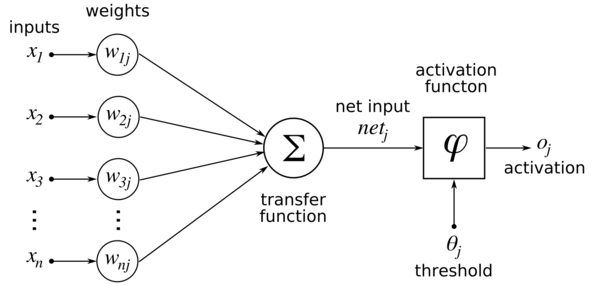
\includegraphics[width=\textwidth]{immagini/pictures/neuron.png} 
\caption{Visual representation of the activation function that determines a neuron's output and the parameters that influence it.}
\end{center}
\end{figure}	

\begin{figure}[htbp]
\begin{center}
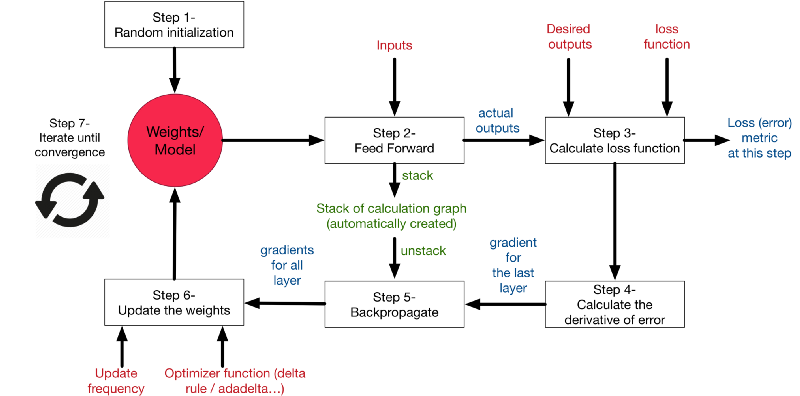
\includegraphics[width=\textwidth]{immagini/pictures/training.png} 
\caption{Schematic representation of how a network updates the weight to decrease the loss and achieve better accuracy.}
\end{center}
\end{figure}
	
\section{Deep neural networks}
	As mentioned above, the \emph{deep learning} approach to solve a problem is to train a \emph{deep neural network} to recognize the wanted features so it can later make predictions about them. Basically when you train a \emph{deep neural network} you feed it thousands of data samples, so it can learn from the wanted data representation by "seeing" it, just like you would show a child pictures of kittens to teach him what a kitten is.
	There are two different ways to train a network, each one with different goals and contexts of use:
	\begin{itemize}
		\item supervised training: the network is given a labeled \emph{\gls{dataset}}\textsubscript{g} to learn from; for each data sample the ground truth is provided, so the network knows what it is learning. This is the preferred approach whenever labeled data is available.
		\item unsupervised training: the network is given an unlabeled \emph{dataset} to learn from; no ground truth is given, so the network has to identify patterns and divide them into different categories on its own. This approach is preferred when the goal is to group data in categories or when data is too complex to be labeled.
	\end{itemize}
	There are different network architectures, each one dedicated to a specific type of problems. When solving  \emph{\gls{computer vision}}\textsubscript{g} task the best performances are held by a class of networks called \emph{convolutional neural networks}. \\

	\subsection{Convolutional neural networks}
	\emph{convolutional neural networks} (CNNs) are \emph{deep neural networks} that consist of an input layer, an output layer, and a variable number of hidden layers with different purposes. What names this family of networks is in fact on particular type of layer, called \emph{convolutional layer}; a single network typically contains various \emph{convolutional layers} of different size, and each perform a \emph{convolution} operation that filters its input stimuli before passing them the to next layer in order to reduce the parameters number, thus allowing the network to be deeper. \\
	CNNs, among others, are mainly used to perform computer vision tasks; in particular they achieve good results in object detection tasks. \\

\begin{figure}[htbp]
\begin{center}
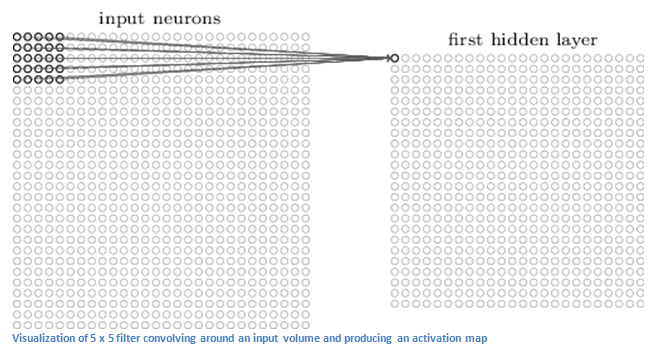
\includegraphics[width=\textwidth]{immagini/pictures/ActivationMap.png} 
\caption{Visual representation of a convolutional layer.}
\end{center}
\end{figure}

	\subsection{Object detection}
	\emph{Object detection} is a computer vision problem that concerns the identification of class instance objects in an image (or video), and locating the actual position of said object in the picture. Commonly the spacial orientation of the detected object is framed by a rectangular \emph{bounding box} that determines its height and width. Thus, object detection is far more powerful than mere image classification, not only because it "draws" a box where the object is located, but also because it can identify multiple object instances in a single image, while classification models have the limit of labeling only the one predominant object in the scene. The capability of labeling and locating multiple instances opens object detection models to a new set of application, such as video surveillance (e.g. moving subjects can be tracked) and instance counting for industrial purposes (e.g. counting boxes in a warehouse). Furthermore, object detection has proven to be more reliable than classification to scan images where the subject of interests occupies only a small part of the picture (e.g. a street sign in the corner). \\
	Commonly an \emph{object detection} model is actually built on top a classifier that works as a \emph{feature extractor}, but this exudes the topics of my project and I am introducing this notion only because it is noticeable in the naming convention of model networks, which are indeed important in my work. \\
	There are three popular network architectures for object detection:
	\begin{itemize}
		\item SSD (Single Shot Detection);
		\item R-CNN (Region-based \emph{convolutional neural network}, and its upgrades Fast R-CNN and Faster R-CNN);
		\item YOLO (You Only Look Once).
	\end{itemize}
While both \emph{SSD} and \emph{YOLO} follow the same approach of computing the image data through a single network, \emph{R-CNN} splits the image in various regions trying to guess where objects of interest might be and processes each area separately, thus requiring more computational power. State-of-the-art models share comparable performances in accuracy, but due to the time overhead of processing a picture multiple times, \emph{R-CNN} is a bit slower than \emph{SSD} and \emph{YOLO}.

\begin{figure}[htbp]
\begin{center}
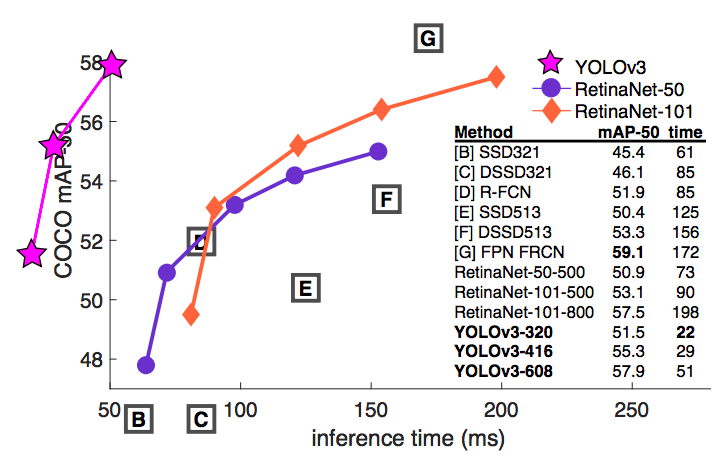
\includegraphics[width=\textwidth]{immagini/pictures/netcomparison.png} 
\caption{Comparison on object detection performances on Nvidia Titan X GPU. A higher mAP value means a better accuracy.}
\end{center}
\end{figure}

\subsection{YOLO v3}
	\emph{YOLO}\footnote{\url{https://pjreddie.com/darknet/yolo/}} is a \emph{convolutional neural network} built on top of \emph{Darknet} classifier, now on its third version \emph{YOLO v3}. Both \emph{YOLO} and \emph{Darknet} are developed by Joseph Redmon on his C-written open source neural network framework Darknet\footnote{To avoid misunderstandings I will call Darknet the framework and \emph{Darknet} the classifier.}. \\
	What makes \emph{YOLO} stand out compared to its competitor is its speed: at par of accuracy YOLO can perform inference in less than half the time, achieving the ability to track moving subjects in real time in 30fps videos using a gaming-tier GPU\footnote{Real time inference is possible on Nvdia GeForce Titan X GPU.}. \\
	For my project I was asked to used \emph{YOLO} in its newest version, \emph{YOLO v3}. As I already said, \emph{YOLO} was firstly implemented in Joseph Redmon's Darknet framework, which is written in C so it is fast, but unfortunately it is suitable only for research purposes. Since I was asked to develop a production-ready application, I had to choose another framework to work on, and I will discuss about it in later chapters.
	
	\subsubsection{Structure}
	\emph{YOLO v3} is an \emph{convolutional neural network} for \emph{object detection} built on top of \emph{Darknet53}, an image classifier that uses 53 convolutional layers. With \emph{Darknet53} as its feature extractor, \emph{YOLO}  processes every image once, looking at it as a whole, hence encoding extra information about the context each class lives in. To do so it models detection as a regression
problem, dividing the image into an S $\times$ S grid, and for each grid cell predicts B bounding boxes, confidence for those boxes, and C class probabilities; when a class-object's center falls inside a grid cell, that grid cell is responsible of detecting that object.
	

\begin{figure}[htbp]
\begin{center}
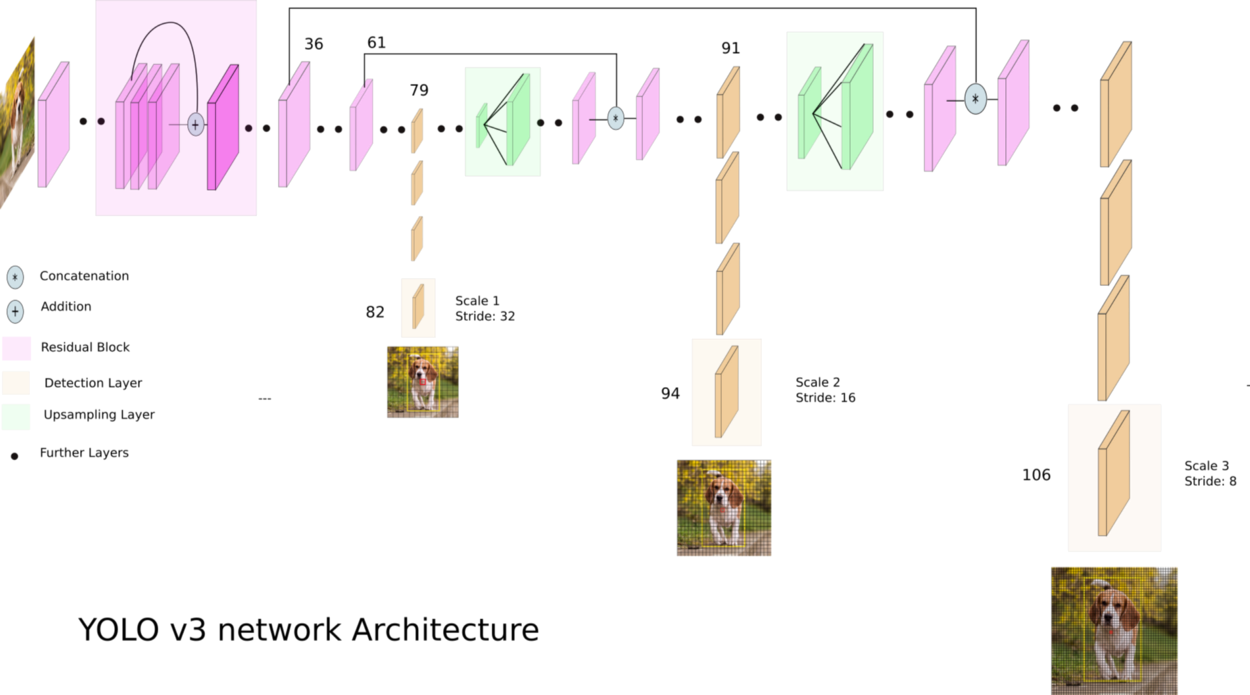
\includegraphics[width=\textwidth]{immagini/pictures/yoloworkflow.png} 
\caption{Workflow of how a \emph{YOLO v3} network processes an image, making it pass through its layers.}
\end{center}
\end{figure}
	
\section{Training a network}
	Training a \emph{convolutional neural network} is a computation-heavy task, that involves the processing of thousands of pieces of data, which in the context of computer vision is in the format of images. Therefore best way to process thousands of images is to use a GPU; using a GPU (or even clusters of GPUs) it is possible to process the images in parallel among the \emph{cores}, speeding up the process greatly. As a comparison, while training on CPU would take days even on a small dataset, on a GPU all the work would be done in just few hours.
	
	\subsection{Dataset}
	The first and most important step to train a network is to create the \emph{dataset} it will learn from. Note that the quality of the dataset itself will have great influence on the final accuracy of the network. For instance you will want to feed your network examples of your objects of interest from every perspective and immerse in their context; also, when training a network to perform an \emph{object detection} task, you want your \emph{bounding boxes} to be as accurate and tight around the figures as possible. \\
	Clearly, creating a custom dataset is a demanding job, since piece of data must be manually labeled by a human. For my project I was given a custom dataset created by one of my colleagues, containing classes relevant for one of THRON's clients. Creating a \emph{dataset} exudes the goals of my project, since on production it will be possibly performed by clients\footnote{As explained in the introduction, THRON's product is a DAM, which in this context can basically seen as a database of categorized images; with possibly minor changes to data labeling (e.g. introduction of bounding boxes for the objects of interest) and database export, image data can be easily turned into a dataset for computer vision.}. \\
	When creating an \emph{object detection} \emph{dataset} there are there are two main qualities to determine its goodness:
	\begin{itemize}
		\item \emph{Cardinality}, which is the means of the number of labels per image;
		\item \emph{Density}, which is the cardinality divided by the number of classes.
	\end{itemize}
A density too low has negative influence on the final accuracy of the network, because basically you are trying to teach it to recognize a high number of classes, but you're giving it only a few examples for each. On a lesser degree, a cardinality too high has  a negative influence on the final accuracy as well because the examples you are giving are too cluttered with information. Furthermore, when creating your own \emph{dataset}, you might want to insert a similar amount image samples/labels for each class. \\
After the full dataset is created, it is common practice to divide it into two separate \emph{datasets}: a \emph{training dataset} and a \emph{validation dataset}, with the suggested ratio of 70\% training and 30\% validation. Note that these two \emph{datasets} contain different samples to avoid \emph{\gls{overfitting}}\textsubscript{g}.

	\subsection{Training}
	Once the dataset is ready and formatted in the network's preferred format\footnote{Depending on the framework, the preferred format changes. To work with YOLO v3 on MXNet data can provided in both RecordIO format or LST + Jpeg format.}, the training process can begin. \\
	The training process is conceptually simple; as previously stated, teaching a machine to recognize kittens can be compared to showing pictures to a child and pointing at the kitten in them to make him understand what a kitten is. When doing so with a child you only need a few examples, when with a machine you'll probably need a few hundreds. The next step is to check whether the machine truly learned what a kitten is; again this can be roughly compared to checking whether the child truly learned what a kitten is by giving him a picture and asking him to point at the kitten, if there is one. \\
	Now that we talked about kittens and children we can explore in detail how a machine learns the way a human would.
	The training process is a loop in which the network is "shown" the \emph{dataset} it should learn from; since a \emph{dataset} is composed by thousands of images, it can't be entirely loaded into memory and must be split in smaller units for processing, called \emph{batches}; in practice maximum \emph{batch} size is determined by your hardware specifics. Your network will be fed all of the training \emph{dataset} \emph{batch} after \emph{batch}. Each loop of computation on the whole training dataset is called an \emph{\gls{epoch}}\textsubscript{g}. To train your network you will want to perform at least a couple of hundreds epochs; this means that to learn the \emph{dataset} your network will go through all of it hundreds of times. 

	\subsection{Validation}	
	Every fixed epoch number you will want to check your network's learning progress; to do so you will perform a validation loop, which means that you will feed the network your validation \emph{dataset} and compare the network's prediction with the ground truth. There are various metrics to calculate a network's accuracy, and the one I used on my project is called \emph{\gls{mean average precision}}\textsubscript{g} (mAP). This evaluation metric uses an \emph{\gls{intersection over union}}\textsubscript{g} (IoU) threshold to determine how well the detected positives overlap with the ground truth; setting the IoU threshold higher or lower influences the wanted precision at locating objects\footnote{Note that ground truth bounding boxes are hand-drawn by a human so they already come with an error, thus setting the IoU threshold too high could prove to be useless and even counterproductive.}, and I set it to a value of 0.5.
	
\begin{figure}[htbp]
\begin{center}
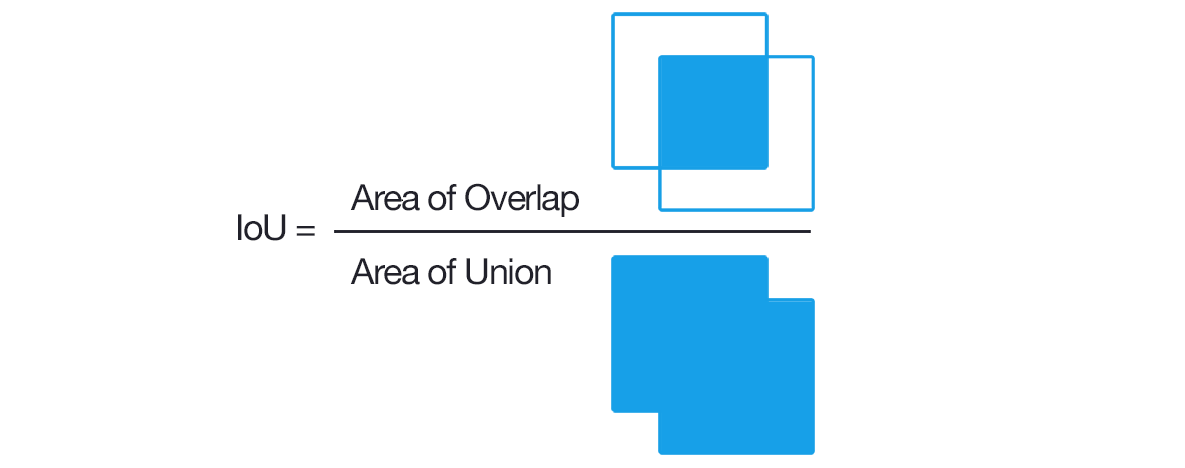
\includegraphics[width=\textwidth]{immagini/pictures/iou_equation.png} 
\caption{Graphic representation of \emph{intersection over union}.}
\end{center}
\end{figure}
	
	\subsection{Transfer learning}
	Training a network from scratch is a quite demanding operation in terms of computational time and power, because the weights for each class need to be calculated from a random initialization. Luckily, it is possible to train a network to recognize new custom classes starting from pre-trained weights for other (general) classes, and this process is called \emph{transfer learning}. \\
	 Basically when you apply transfer learning on a pre-trained network\footnote{All the major deep learning frameworks usually provide networks and weights pre-trained on popular datasets such as COCO, VOC or ImageNet.}, you teach it to recognize new classes by adjusting its weights (which have a meaning and are not random anymore) and the structure of the two layers that determine the final output. To benefit from \emph{transfer learning}
	 you want to choose a base network with weights for classes that share some features with your custom ones for example if you want to be able to detect different species of animals, a good choice would be to \emph{fine-tune} a network trained on a datasets that already contains cats and dogs.
	
	\subsection{Hyperparameters}
	The accuracy of a \emph{convolutional neural network} is influenced by various paramenters, called hyperparameters, that tweak how the weights are updated and how the results are evaluated. This values come in the form of \emph{"magic numbers"}, meaning that for every dataset each network has its own values to optimize the final performance and that they can be found only in a trial and error fashion\footnote{To determinate the best values it is common practice to re-train the network various times and compare the results.}. Since this is rather time consuming, especially when training on CPU, I couldn't tune the hyperparameters for my project. However I will introduce briefly what the main hyperparameters do on a \emph{YOLO v3} architecture network.
	\begin{itemize}
	\item Learning rate. Speed at which the network learns. It is used when updating weights and a learning rate too high might cause overfitting.
	\item Learning rate deacay rate. As the network learns, its learning rate decreases; this value is important to avoid overfitting.
	\item Momentum. Stochastic gradient descent momentum, used by the gradient descent function to calculate how to reduce the loss.
	\end{itemize}

\section{Object detection for THRON}
	As mentioned in Chapter 1, THRON already uses generic classification services in its \emph{DAM}. Therefore, to provide a better service, it comes natural that the Company has interest in developing a system able to detect custom classes. \\
	Since THRON already has a vast database of labeled data, following a deep learning approach is the easiest option, even more so now that framework providing almost out-of-the-box are increasing prominence. \\
	At first it was still unclear whether the Company needed just a classifier, but with my proof-of-concept the benefits of an \emph{object detection} model became clear. We particularly chose \emph{YOLO v3} under the suggestion of a data scientist working in my team, since he already developed a research-purpose prototype application using \emph{YOLO v2}. Due to the technology used, his application couldn't be released in a production environment, so it was my job to develop a production-ready application using \emph{YOLO}.             % Processi
% !TEX encoding = UTF-8
% !TEX TS-program = pdflatex
% !TEX root = ../tesi.tex

%**************************************************************
\chapter{Internship description}
\label{chap:internship-description}
%**************************************************************

\intro{My project at THRON S.p.A. was to develop a production-ready application for \emph{object detection} using \emph{YOLO v3}. I was given the responsibility to choose the framework to use, and I coded both the training and inference parts of the application.}\\

%**************************************************************
\section{Project introduction}
The goal of my project was to develop a production-ready \emph{object detection} application that could be integrated in Thron in the future. Since THRON strongly relies on web services like those provided by \emph{\gls{AWS}}\glsfirstoccur, so it was my job to keep compatibility.
%**************************************************************
\section{Risk analysis}

Every project comes with its risks. Since deep learning is a relatively new field, my project was at high risk from the beginning.\\

\begin{center}
    \begin{tabular}{ | p{5cm} | p{5cm} | p{2cm} |}
    \hline
    \textbf{Decription} & \textbf{Solution} & \textbf{Occurrence} \\ \hline
    \textbf{Stable release} \\ The technology I used is fairly new, so it is not surprising that the main toolkit I used was in version 0.3.0 (version 0.4.0 was released later on my internship). This lead to some inconveniences such as bugs and inconsistencies between documentation and source code. & No real solution was identified. When necessary I submitted issues to the code developers and patched bugs myself when I could. & High \\ \hline
    \textbf{AWS support}\\ Since the technology I used was fairly new, it relied on the newest version of my framework of choice. During my AWS provided out-of-the-box support only to the previous version of my chosen framework, which isn't compatible with the core toolkit I used. & No real solution was identified. I tried other AWS services, but they are not as straightforward as the one I was supposed to use and proved to be rather troublesome. & High \\ \hline
    \textbf{Hardware} \\ Deep learning is a demanding technology that requires a lot of computational power. Specifically, it is suggested to execute training on a GPU since it is much faster, but I didn't have one. Training on CPU, on the other hand, is indeed possible, but it requires fairly new hardware, which, during my first week, I didn't have. & Before I was assigned a newer CPU I got to work on a remote AWS machine via SSH. This machine provided a GPU so I could test example algorithms. When given a newer CPU I had to train my network on that, which required a couple of days and thus prevented me from tuning the hyperparameters. & High \\ \hline
   \textbf{Python} \\ Deep learning frameworks are written almost exclusively in Python. With no prior experience, writing a Python application could prove to be troublesome. & None of my coworkers was a Python expert, but they always helped me to find good libraries and frameworks to use. & Medium \\ \hline
   \end{tabular}
\end{center}


%**************************************************************
\section{Requisiti e obiettivi}


%**************************************************************
\section{Pianificazione}             % Kick-Off
%% !TEX encoding = UTF-8
% !TEX TS-program = pdflatex
% !TEX root = ../tesi.tex

%**************************************************************
\chapter{Analisi dei requisiti}
\label{cap:analisi-requisiti}
%**************************************************************

\intro{Breve introduzione al capitolo}\\

\section{Casi d'uso}

Per lo studio dei casi di utilizzo del prodotto sono stati creati dei diagrammi.
I diagrammi dei casi d'uso (in inglese \emph{Use Case Diagram}) sono diagrammi di tipo \gls{uml} dedicati alla descrizione delle funzioni o servizi offerti da un sistema, così come sono percepiti e utilizzati dagli attori che interagiscono col sistema stesso.
Essendo il progetto finalizzato alla creazione di un tool per l'automazione di un processo, le interazioni da parte dell'utilizzatore devono essere ovviamente ridotte allo stretto necessario. Per questo motivo i diagrammi d'uso risultano semplici e in numero ridotto.

\begin{figure}[!h] 
    \centering 
    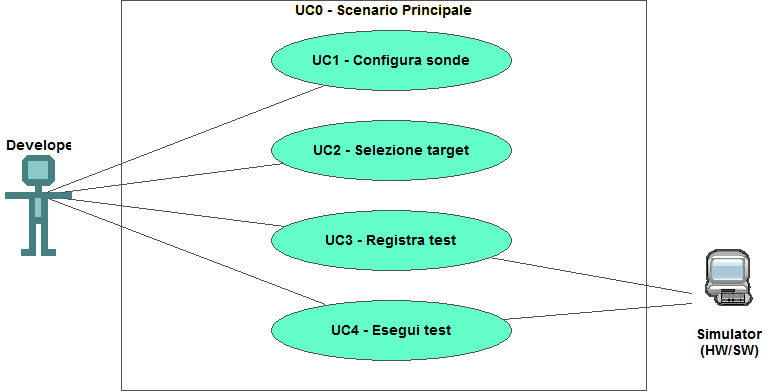
\includegraphics[width=0.9\columnwidth]{usecase/scenario-principale} 
    \caption{Use Case - UC0: Scenario principale}
\end{figure}

\begin{usecase}{0}{Scenario principale}
\usecaseactors{Sviluppatore applicativi}
\usecasepre{Lo sviluppatore è entrato nel plug-in di simulazione all'interno dell'IDE}
\usecasedesc{La finestra di simulazione mette a disposizione i comandi per configurare, registrare o eseguire un test}
\usecasepost{Il sistema è pronto per permettere una nuova interazione}
\label{uc:scenario-principale}
\end{usecase}

\section{Tracciamento dei requisiti}

Da un'attenta analisi dei requisiti e degli use case effettuata sul progetto è stata stilata la tabella che traccia i requisiti in rapporto agli use case.\\
Sono stati individuati diversi tipi di requisiti e si è quindi fatto utilizzo di un codice identificativo per distinguerli.\\
Il codice dei requisiti è così strutturato R(F/Q/V)(N/D/O) dove:
\begin{enumerate}
	\item[R =] requisito
    \item[F =] funzionale
    \item[Q =] qualitativo
    \item[V =] di vincolo
    \item[N =] obbligatorio (necessario)
    \item[D =] desiderabile
    \item[Z =] opzionale
\end{enumerate}
Nelle tabelle \ref{tab:requisiti-funzionali}, \ref{tab:requisiti-qualitativi} e \ref{tab:requisiti-vincolo} sono riassunti i requisiti e il loro tracciamento con gli use case delineati in fase di analisi.

\newpage

\begin{table}%
\caption{Tabella del tracciamento dei requisti funzionali}
\label{tab:requisiti-funzionali}
\begin{tabularx}{\textwidth}{lXl}
\hline\hline
\textbf{Requisito} & \textbf{Descrizione} & \textbf{Use Case}\\
\hline
RFN-1     & L'interfaccia permette di configurare il tipo di sonde del test & UC1 \\
\hline
\end{tabularx}
\end{table}%

\begin{table}%
\caption{Tabella del tracciamento dei requisiti qualitativi}
\label{tab:requisiti-qualitativi}
\begin{tabularx}{\textwidth}{lXl}
\hline\hline
\textbf{Requisito} & \textbf{Descrizione} & \textbf{Use Case}\\
\hline
RQD-1    & Le prestazioni del simulatore hardware deve garantire la giusta esecuzione dei test e non la generazione di falsi negativi & - \\
\hline
\end{tabularx}
\end{table}%

\begin{table}%
\caption{Tabella del tracciamento dei requisiti di vincolo}
\label{tab:requisiti-vincolo}
\begin{tabularx}{\textwidth}{lXl}
\hline\hline
\textbf{Requisito} & \textbf{Descrizione} & \textbf{Use Case}\\
\hline
RVO-1    & La libreria per l'esecuzione dei test automatici deve essere riutilizzabile & - \\
\hline
\end{tabularx}
\end{table}%             % Concept Preview
% !TEX encoding = UTF-8
% !TEX TS-program = pdflatex
% !TEX root = ../tesi.tex

%**************************************************************
\chapter{Design and development}
\label{cap:design-development}
%**************************************************************

\intro{In this chapter I will explain my technology choices and how these influenced the development of the final application.}\\

%**************************************************************
\section{Technology and tools}
\label{sec:technology-tools}

In the following I will introduce the technologies I used and the reasons behind their choice.

\subsection*{Deep learning framework}
There are many popular deep learning frameworks out there, but I was asked to choose between \emph{MXNet} and \emph{TensorFlow} after experimenting with both for bit. Keep in mind that I was required to use \emph{YOLO v3} as my \emph{convolutional neural network} and it influenced greatly my final choice. Furthermore, due to Python being predominant in deep learning, I had little freedom in choosing a programming language\footnote{Actually I did try Scala APIs on MXNet, but I had little success with them due to the restricted set of functionality provided when compared to Python.}

\subsubsection*{MXNet and Gluon CV}
\emph{MXNet} is an open source deep learning framework developed by Apache. It supports various languages, but the most extensive toolkit is written in Python; in particular MXNet Python provides \emph{Gluon}, a high-level API that allows to easily build and train \emph{deep neural networks}. \emph{Gluon} is also used by \emph{Gluon CV}, a \emph{computer vision} toolkit that provides out-of-the-box implementation of several \emph{neural networks}, pre-trained models and even complete \emph{training scripts}. In particular \emph{YOLO v3} is well supported and many useful tutorials are available. \\
Both \emph{MXNet} and \emph{Gluon CV} can be installed from \emph{\gls{PyPI}}\textsubscript{g} with \emph{\gls{Pip}}\textsubscript{g}. \\
There are minor compatibility issues since \emph{Gluon CV} 0.3.0 requires \emph{MXNet} 1.3.0 and later.

\subsubsection*{TensorFlow}
\emph{TensorFlow} is an open source machine learning framework developed by Google Brain. It supports various language, but as common in this field the most extensive one is written in Python. \emph{TensorFlow} is compatible with \emph{Keras}, a high-level API to build and train \emph{deep neural networks}; sadly \emph{Keras} does not provide any network model for \emph{computer vision}. \\
When looking to \emph{YOLO v3} support I explored \emph{TensorFlow}'s \emph{GitHub} repository, where they host some research projects developed and maintained by independent researchers and not officially supported or distributed in release branches. Among the \emph{computer vision} models on there I did not find \emph{YOLO v3}, but I took my time to experiment with a \emph{SSD} model just to see if \emph{TensorFlow} was worth anyway. \\
\emph{TensorFlow} can be installed from \emph{PyPI} with \emph{Pip}, but the research toolkit cannot.

\subsubsection*{My choice}
Since \emph{MXNet}'s \emph{Gluon CV} provides a comprehensive toolkit with models, scripts and utilities to train and infer \emph{YOLO v3} \emph{convolutional neural networks}, it easily became my framework of choice. \\
As I said I tried \emph{TensorFlow} with \emph{SSD}, but it was a low-level implementation that relied a lot on a \emph{\gls{Jupyter notebook}}\textsubscript{g} and it was not suitable for the goals of my project.

\subsection*{IntelliJ IDEA}
I used \emph{\gls{IntelliJ IDEA}}\textsubscript{g} IDE to write my code and I installed \emph{PEP} \emph{Python} linter plugin to check my code style. \\


\subsection*{GitLab}
I was given access to a \emph{\gls{GitLab}}\textsubscript{g} repository to version control my work and I used \emph{IntelliJ IDEA}'s built-in \emph{Git} interface to access it.


\subsection*{Docker}
\emph{\gls{Docker}}\textsubscript{g} is a software application to create containers, virtual environments with their own operative system and tools installed. Containers can communicate with each other and to the outer world through ports, and can mount hard drives when consistent memory is needed. \\
I used it in various steps of my project's development; at first I created a \emph{Linux} \emph{Docker} container to set up a \emph{Python 2.7} and \emph{MXNet} environment to run my code. I also created a \emph{MongoDB} instance on another container. \\
At some point I even dockerized my application to run it on \emph{AWS}.


\subsection*{OpenAPI + Swagger}
Thron works with a service architecture, so I was asked to follow it when developing my inference web application. I wrote a \emph{\gls{YAML}}\textsubscript{g} \emph{\gls{OpenAPI}s}\textsubscript{g} using \emph{\gls{Swagger}}\textsubscript{g} to declare my application's interface, which also served as documentation.

\subsection*{Flask + Connexion}
My server application for inference is written in \emph{Python}, so I set up a \emph{\gls{Flask}}\textsubscript{g} server to host it. The \emph{Flask} needed to adhere to the operations and responses I declared on the \emph{OpenAPI}; matching everything manually would be a tedious job, but thankfully \emph{Zalando}\footnote{E-commerce platform.} developed a framework called \emph{Connexion}\footnote{Zalando Connexion repository: \url{https://github.com/zalando/connexion}} that, provided the \emph{OpenAPI} automatically handles the HTTPs requests and maps them to your Python functions.

\subsection*{Postman}
I used \emph{\gls{Postman}}\textsubscript{g} to send \emph{HTTP} request to my web server and check its behavior.

\subsection*{MongoDB + Robo 3T}
I set up a \emph{\gls{MongoDB}}\textsubscript{g} instance in a \emph{Docker} container to model a queue I needed in my inference application, and I used the \emph{Pymongo}\footnote{Pymongo website: \url{https://api.mongodb.com/python/current/}} toolkit to work with it from my server application. \\
To easily access and manage my database, I used \emph{\gls{Robo 3T}}\textsubscript{g} client.

\subsection*{AWS SageMaker}
I experimented with \emph{AWS} \emph{\gls{SageMaker}}\textsubscript{g} to test whether a \emph{YOLO v3} training script could easily take advantage of \emph{AWS}'s computational power in a future production environment.




%**************************************************************


%**************************************************************
\section{Design}
\label{sec:design}
In this section I will cover the design choices I made while developing my application.

\subsection{Overview}
As stated before, THRON'S \emph{DAM} categorizes images inserted by the clients to make their access easier. Details about how these images are stored in a non-relational database are irrelevant for my project, and I actually do not know them. However, how a database export is structured and what it contains do is important and had major influence in some implementation choices. \\
A database export is a  \emph{\gls{Json lines file}}\textsubscript{g} where each line represent a valid Json file containing information about an image in the database; the covered fields are the following:
\begin{itemize}
	\item ID: image unique identifier;
	\item Client ID: client identifier\footnote{Thron has several clients and often uses client ID based sharding techniques to run services in order to guarantee various levels of fairness.}; the goal is to construct a custom dataset for detection for each client's needs so this parameter is vital;
	\item Url: location where the image is stored, likely an \emph{Amazon S3}\footnote{AWS cloud storage service; Amazon S3 website: \url{https://aws.amazon.com/s3}} cloud storage location.
	\item Data: image properties relevant in the dataset context such as \emph{bounding boxes} coordinates and classes.
\end{itemize}


\subsection{Dataset creation}

\subsubsection{Format choice}
To train the network model for my prototype I was given a dataset created by one of my co-workers; his format of choice\footnote{Each raw image in the dataset was labeled by an XML file containing the image size, bounding boxed and classes.}, however, it was not compatible with my framework so I had to convert it with a script. \\
\emph{Gluon CV} provides modules to load a custom dataset from two different formats:
\begin{itemize}
	\item Record file format; this format is composed by two different files, a \emph{*.rec} binary file, containing the encoded images and their labels, and a \emph{*.idx} file containing the indexes to provide random access to the binary;
	\item Pure text file format; this format is composed by a \emph{*.lst} file\footnote{It is a text file readable as a tab-separated \emph{*.csv file.}}. Each line of this file contains the path to an image on disk and the labels describing its bounding boxes.
\end{itemize}


\begin{figure}[htbp]
\begin{center}
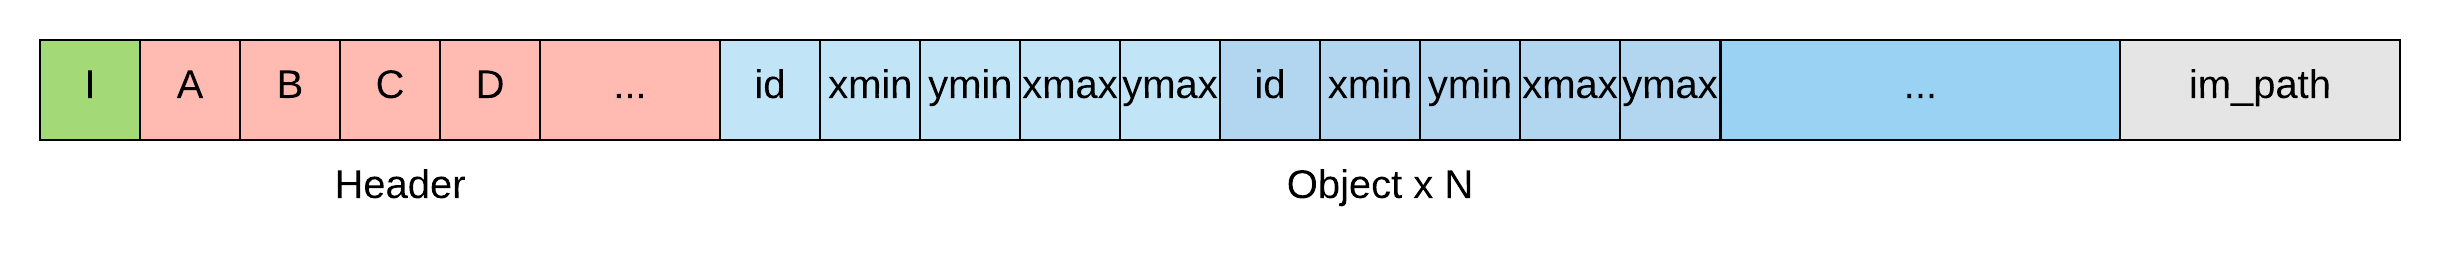
\includegraphics[width=\textwidth]{immagini/pictures/detection_label.png}
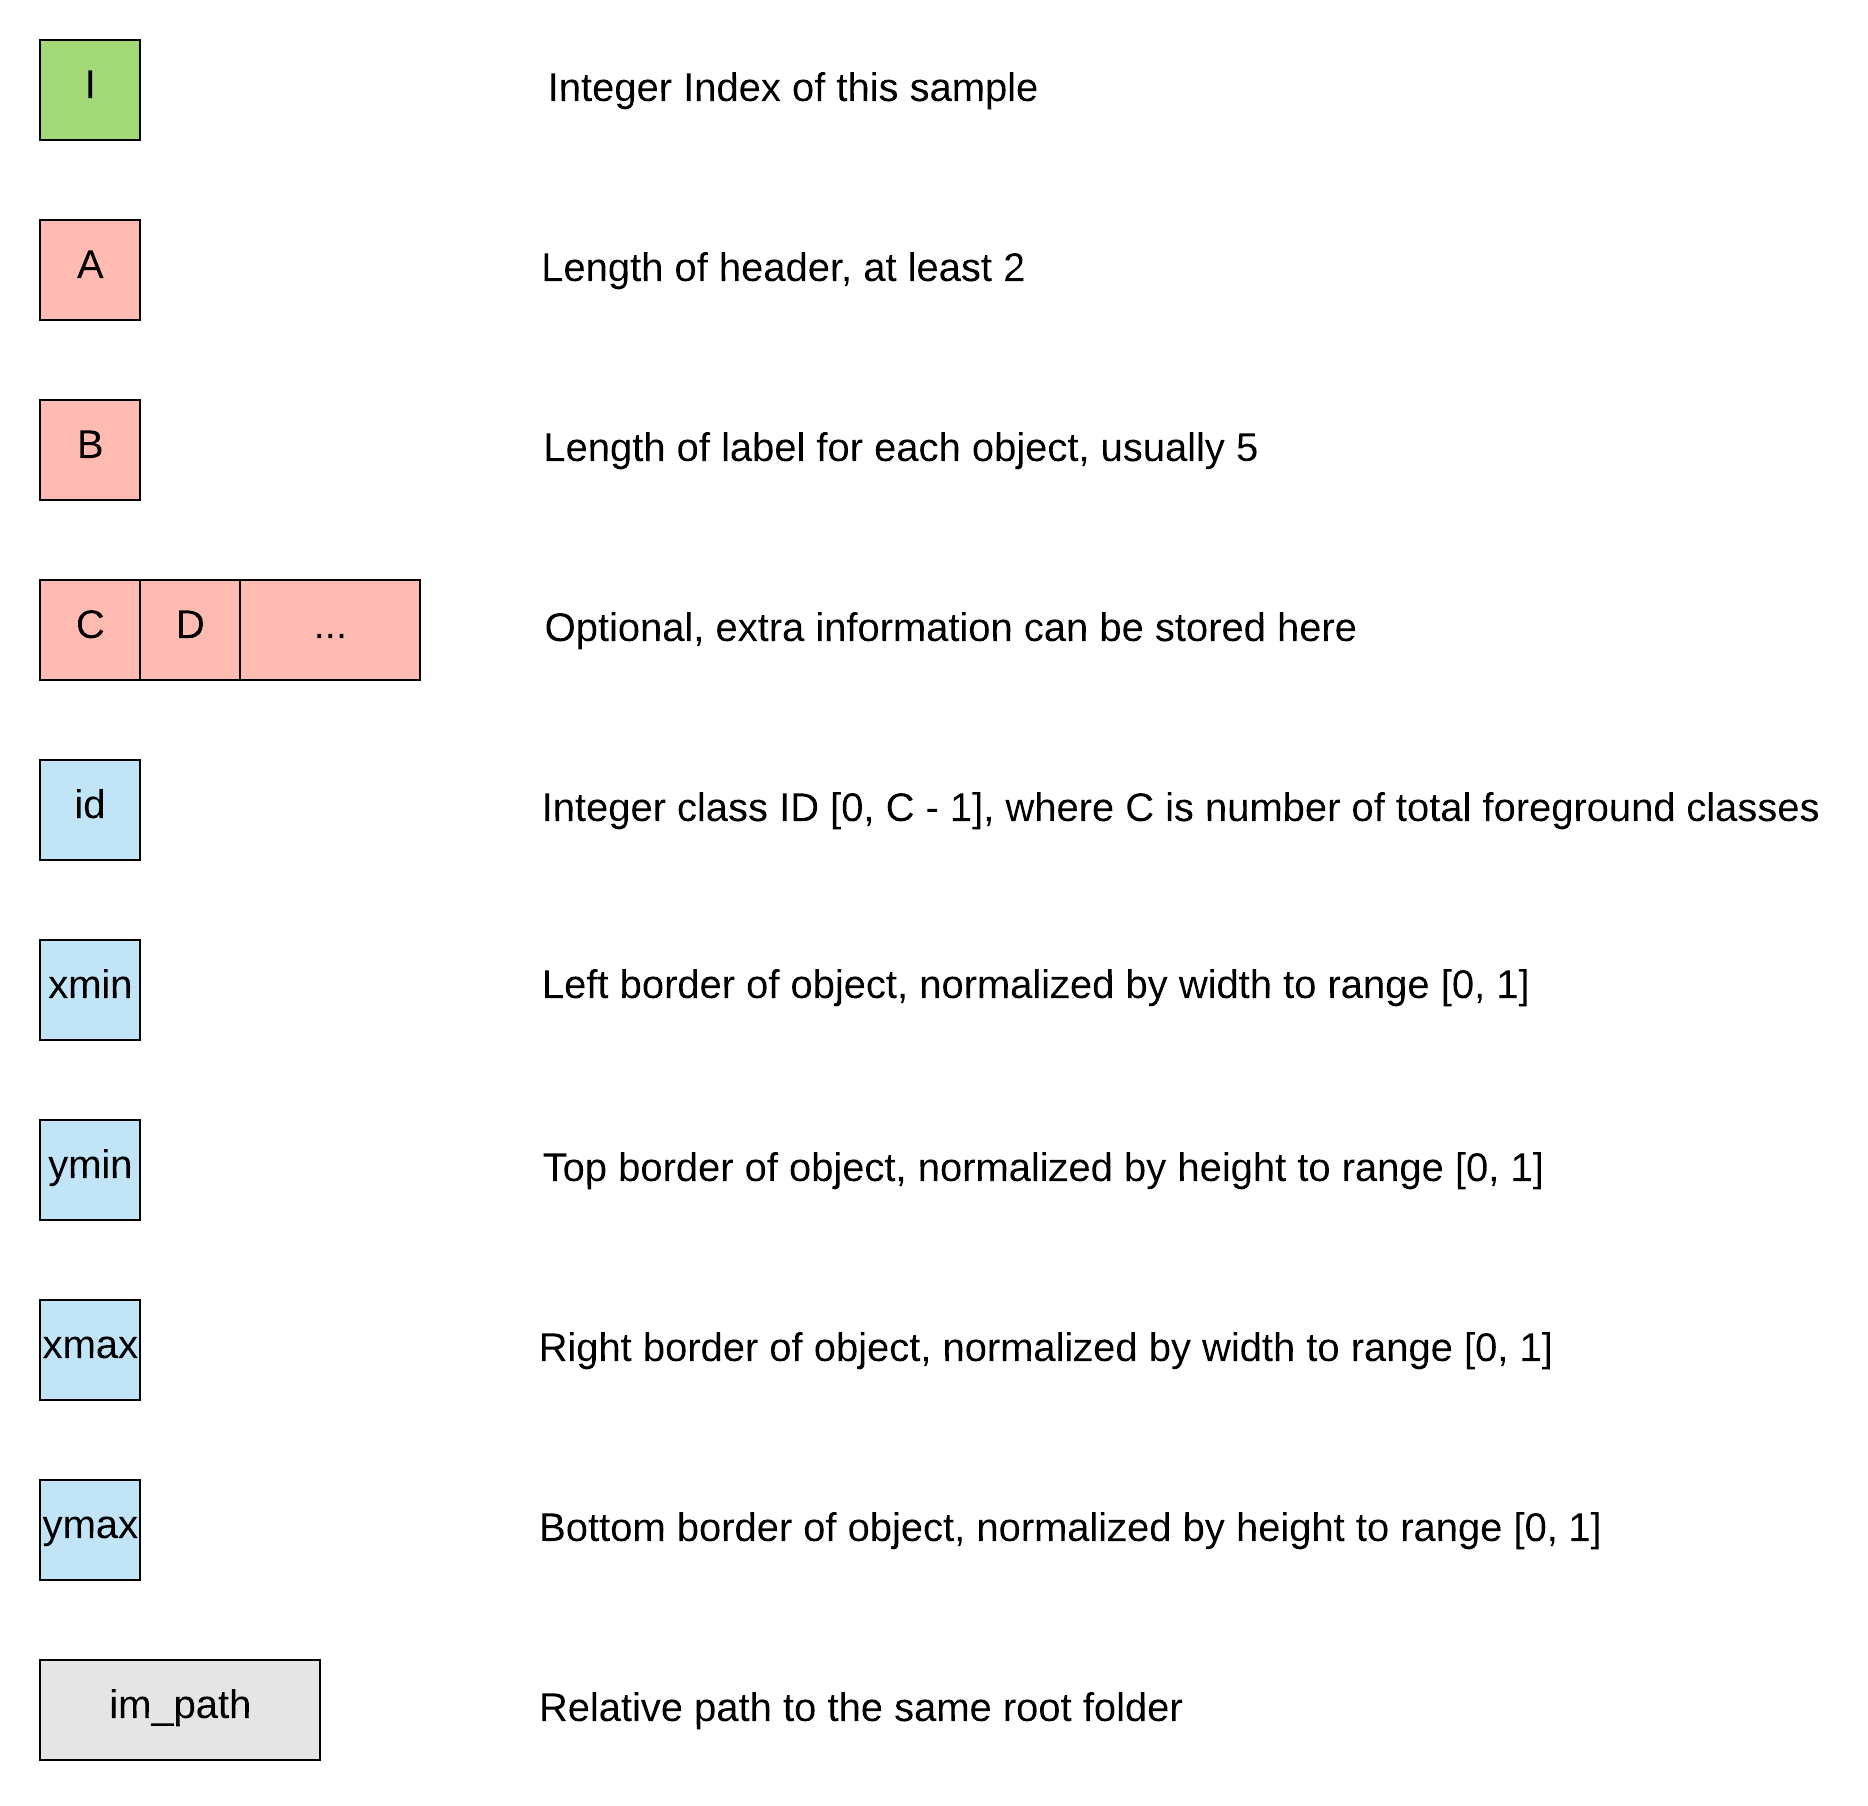
\includegraphics[width=\textwidth]{immagini/pictures/detection_label_detail.png} 
\caption{Structure of a \emph{*.lst} file containing dataset information.}
\end{center}
\end{figure}

The record file format allows faster training, but I chose to use the \emph{*.lst} file format instead because it allows you to work directly from raw images without prior computation. There are two main reason behind my choice:
\begin{enumerate}
	\item The production training process should run on \emph{AWS SageMaker}, which reads input data from an \emph{Amazon S3}; Thron already uses \emph{S3} so uploading the training on a dedicated bucket on there would be the easiest approach;
	\item In production environment the datasets should be created from \emph{Json lines file} database exports, so simply converting the \emph{Json lines} content describing the bounding boxes for each image to an \emph{*.lst} would be the easiest and fastest approach.
\end{enumerate}



\subsubsection{Dataset creation approach}
The dataset-creation module I designed takes a \emph{Json lines} database export file as its input and creates a \emph{*.lst} for each \emph{client ID} found in the \emph{Json lines}. The module also provides a function to split the dataset into \emph{training dataset} and \emph{validation dataset} after creation and saves an additional text file containing statistics about the dataset\footnote{These statistics include number of images, number of classes, cardinality and density.}. I chose to keep the creation of the full dataset and splitting it separated, as it is common practice to split the dataset right before training. \\
To track the class names with their numerical encoding used in the \emph{*.lst} dataset a \emph{*.txt} calles \emph{synset.txt} is used. This file must be created manually.


\subsection{Training}
Model training for my \emph{YOLO v3} network can be executed as a stand-alone \emph{Python} script. This file receives as an input the \emph{training} and \emph{validation} datasets in \emph{*.lst} format and the \emph{synset.txt} file. \\
My script actually performs \emph{transfer learning} instead of training from scratch due to the better performances achievable this way; the base network is a YOLO v3 Darknet53\footnote{YOLO v3 convolutional neural network built on top of a Darket classifier composed by 53 layers} pre-trained on the \emph{VOC} dataset; the \emph{VOC} weights are provided by the \emph{Gluon CV} toolkit and should cover classes general enough to prove useful in most cases.

\subsubsection{Hyperparameters}
My scripts accepts arguments to tune the training \emph{hyperparameters}. Follows the hyperparameters list and their description:
\begin{itemize}
	\item Data shape: input data shape; the shortest side of each image will be resized to match this value. Accepted values are 320, 416 and 608 (32 multiples) and it defaults to 416;
	\item Batch size: number of images in each computing batch. It must be tuned accordingly to your hardware as a batch size to big would trigger a bus error. It defaults to 8 (which works for CPU), but with GPU training you might be able to use a bigger size such as 32;
	\item Workers: number of workers used for training. You must tune it accordingly to your hardware as a number too high might result in a thread error;
	\item Gpus: numbers of the GPUs to use as a comma separated list of integers; to train on CPU leave this argument empty;
	\item Epochs: number of epochs to perform;
	\item Learning rate: speed at which your model learns the dataset content. A high learning rate makes you model learn quicker, but might result in overfitting;
	\item Learning rate decay rate: speed at which your learning rate decays;
	\item Learning rate decay epoch: epoch interval where your learning rate should decrease;
	\item Momentum: stochastic gradient descent momentum;
	\item Syncbn: argument to synchronize devices when training in parallel.
\end{itemize}


\subsubsection{Model export}
There are two ways to export a trained (or partially trained) network:
\begin{itemize}
	\item Saving weights: it is possible to set the network weights as a \emph{*.PARAMS} binary file every set epoch; this type of file is mostly used as a training checkpoint to resume training from later.
	\item Network export: it is possible to set an export epoch where both the network architecture with adjusted top layers and its weights are exported. The network itself is saved as a \emph{*.json} file describing its layers while the weights are saved as a \emph{*.PARAMS} similar to the checkpoint file. These files are coupled and must be used together to load the trained network; this export approach is used when you want to save a model to use for inference, as it can be loaded from different languages other that \emph{Python}.
\end{itemize}

\subsubsection{Resume training}
Since training demands a lot of computational power, it is useful to be able to stop a training process in order to resume it later. The following arguments allows you to load weights from a training checkpoint to resume training:
\begin{itemize}
	\item Resume: path to the \emph{*.PARAMS} binary file containing the training checkpoint;
	\item Start epoch: epoch where training should be resumed.
\end{itemize}
It is important to load a checkpoint \emph{*.PARAMS} binary file to resume training as the model export \emph{*.PARAMS} binary file cannot be loaded without its paired \emph{*.json}.

\subsection{Inference service}
While training usually requires GPU power to speed up the process, inference can be reasonably done on CPU, so I decided to keep my training script and my inference script separated.

\subsubsection{RESTful Architecture}
My inference request server uses a\emph{\gls{RESTful API}}\textsubscript{g} architecture that I designed using the API first approach; specifically, I wrote my \emph{OpenAPIs} using the \emph{Swagger}. To implement my APIs I took advantage of \emph{Zalando}'s \emph{Connexion}, a framework based on \emph{Flask} that tracks the operations declared in the OpenAPI to the application, validates the HTTP request exchange by comparing the actual Json content to what is declared in the API and manages error messages\footnote{Since I used \emph{Connexion} instead of a pure \emph{Flask} server application I couldn't override the standard HTTP error messages}. \\
To increase decoupling I kept my server interface separated from its implementation; in fact operations are declared in a \emph{JobOpsMongo} module called by the server interface via a \emph{JobService} module. I followed this decoupling approach for both \emph{MongoDB} related operations and \emph{MXNet} inference related operations, but the latter aren't directly called by the inference request server but are used by a queue consumer I did not implement and that potentially resides on AWS.

\begin{figure}[htbp]
\begin{center}
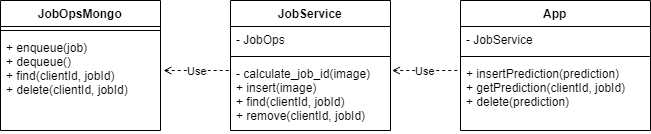
\includegraphics[width=\textwidth]{immagini/pictures/jobops.png} 
\caption{UML describing the relationship between the server application (App class) and the implementation of its methods.}
\end{center}
\end{figure}

Basically the server's job is to accept and manage inference requests by inserting them into a \emph{MongoDB} queue; from there a consumer will dequeue them and run the actutal inference. \\
HTTP requests work with \emph{Json} objects which, despite \emph{Connexion}'s automatic conversion into \emph{Python} dictionaries, still require tedious syntax to access their fields. On the other hand \emph{MongoDM} indexes its content in \emph{Json} format.
Since working with different formats of data would unnecessarily increase the application's complexity, I found it useful to model \emph{Python} class objects to reflect what was declared in the \emph{OpenAPI} and use them to work within the logic modules. My approach while designing these classes was to roughly follow the structure I declared in the OpenAPI, adding further information that could be useful inside the application, and to provide object creation, serialization\footnote{From \emph{Python} object to \emph{Json}} and deserialization \footnote{From \emph{Json} to \emph{Python} objects.} methods to quickly convert between  \emph{Python} objects, \emph{Python} dictionaries and \emph{Json}s as needed. \\

\subsubsection{Asynchronous computation}
While inference isn't to heavy on the computational side of the task, performing a prediction requires the trained network model to be loaded into memory and, since each model occupies over 250MBs of space, it is obvious that constantly switching from model to model would make the performance fall. The easiest solution to this problem is to perform inference by sharding the requests by client ID, so each batch of images runs on the same network model. A further advantage of client ID sharding is that it allows guarantee different levels of fairness accordingly to each client's service contract. \\
Since computation is obviously performed asynchronously, a client needs a way to retrieve its inference once it's completed. There are two main options to manage this: \emph{\gls{callback}s}\textsubscript{g} and \emph{\gls{polling}}\textsubscript{g}. I chose the latter because it comes more natural when working in a \emph{RESTful} environment, as after having inserted the new job in the queue the server can simply send a HTTP 202 Accepted response containing the address to check for the requested resource.

\subsubsection{Queue}
I modeled the queue on \emph{MongoDB}, as it provides an easy way to sort the elements in its collections by insertion time. Furthermore, contents in \emph{MongoDB} are represented as \emph{Json} objects, so it proved to be convenient to work with the objects I declared in the \emph{OpenAPI}. \\
The jobs queue is accessed by both my inference request server and a consumer, but I did not implement the latter.

\subsubsection{Inference work flow}
When a client needs an image to be inferred, it sends the server a HTTP Post request containing a \emph{Json} stating the URL to the image and a client ID; upon receiving the request the server creates a new inference request job and inserts it in a \emph{MongoDB} queue. If the insertion was successful, the server sends the client a HTTP 202 Accepted response, containing the URL where to check for the requested prediction; since computation runs asynchronously, the client might have to check several times for its requested inference result before it's actually available. \\
When the prediction is ready, the client can retrieve it from the given URL; inference contains the detected object classes, their confidence score\footnote{How much the network is confident the detected object belongs to the stated class; a higher score means higher confidence.} and their \emph{bounding boxes}, expressed in percentage on the image's size. \\
Predictions are executed by I consumer I did not implement.

\begin{figure}[htbp]
\begin{center}
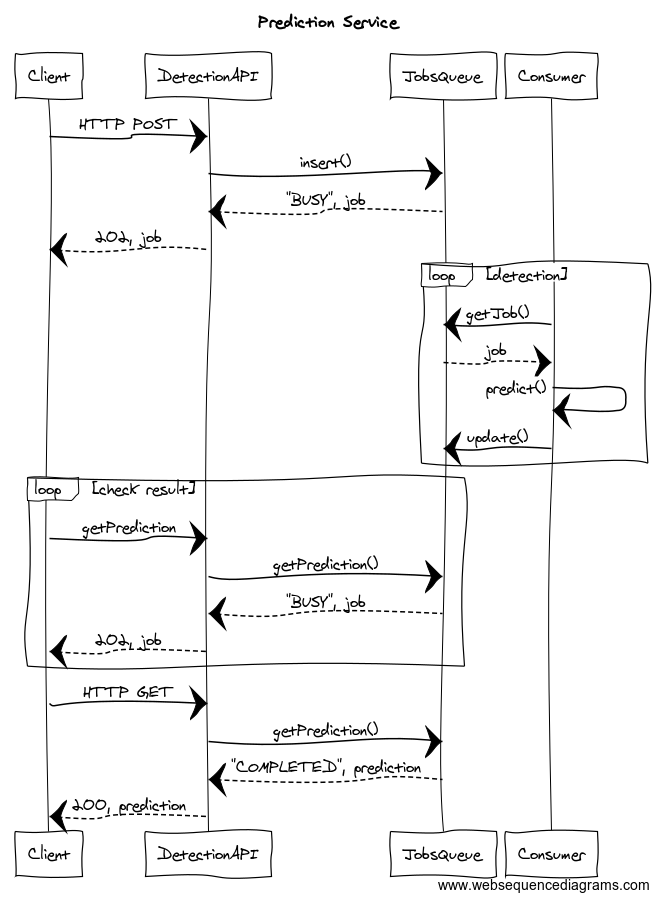
\includegraphics[width=\textwidth]{immagini/pictures/flow.png} 
\caption{UML flow chart displaying the HTTP message exchange in the application.}
\end{center}
\end{figure}


\subsubsection{Unit test}
I wrote unit tests that cover both the methods provided by the \emph{JobOpsMongo} module and the \emph{PredictionOpsMxnet} modules. 
While the \emph{JobOpsMongo} module was actually used by the application and I tried its functionality by sending HTTP requests via \emph{Postman} as well, the \emph{PredictionOpsMxnet} module has only been used by its unit tests. In fact, the \emph{PredictionOpsMxnet} module provides the inference methods that the consumer should use, but I did not implement it because it should potentially run on \emph{AWS} and therefore requires specific coding.

\subsection{Standalone inference script}
Before designing and developing the inference request server application, I wrote a \emph{Python} standalone script to perform inference on an image. This script takes the image path and the network model to use as arguments, and then run inference. The result is composed by the classes of the detected objects, their \emph{bounding boxes} and their confidence score; furthermore the inference script saves a copy of the input image where it draws\emph{To edit images I used Python PILLOW library. PILLOW website: \url{https://pillow.readthedocs.io/en/5.3.x/}} the \emph{bounding boxes} with their class and confidence score. \\
I used this inference script mainly when testing whether the network training was successful; since I used unlabeled data\footnote{Using dataset images for testing could give false performance, especially if overfitting has occurred.} for testing, visually checking whether the detection was accurate proved to be faster that automatizing the process, as classes and their \emph{bounding boxes} must be manually determined by a human anyway.
%**************************************************************

             % Product Prototype
% !TEX encoding = UTF-8
% !TEX TS-program = pdflatex
% !TEX root = ../tesi.tex

%**************************************************************
\chapter{Verifica e validazione}
\label{cap:verifica-validazione}
%**************************************************************             % Product Design Freeze e SOP
% !TEX encoding = UTF-8
% !TEX TS-program = pdflatex
% !TEX root = ../tesi.tex

%**************************************************************
\chapter{Conclusioni}
\label{cap:conclusioni}
%**************************************************************

%**************************************************************
\section{Consuntivo finale}

%**************************************************************
\section{Raggiungimento degli obiettivi}

%**************************************************************
\section{Conoscenze acquisite}

%**************************************************************
\section{Valutazione personale}
             % Conclusioni
\appendix                               
% !TEX encoding = UTF-8
% !TEX TS-program = pdflatex
% !TEX root = ../tesi.tex

%**************************************************************
\chapter{Appendice A}
%**************************************************************

\epigraph{Citazione}{Autore della citazione}



             % Appendice A

%**************************************************************
% Materiale finale
%**************************************************************
\backmatter
\printglossaries
% !TEX encoding = UTF-8
% !TEX TS-program = pdflatex
% !TEX root = ../tesi.tex

%**************************************************************
% Bibliografia
%**************************************************************

\cleardoublepage
\chapter{Bibliografia}

\nocite{*}
% Stampa i riferimenti bibliografici
\printbibliography[heading=subbibliography,title={Riferimenti bibliografici},type=book]

% Stampa i siti web consultati
\printbibliography[heading=subbibliography,title={Siti web consultati},type=online]


\end{document}
